\documentclass{standalone}
\usepackage{tikz}
\usepackage{sansmath}

\usetikzlibrary{shapes.geometric,positioning,calc,petri,graphs}
\tikzset{
        node distance=1.5cm and 2.0cm,
        >=latex,
        font=\sf\bfseries\sansmath,
        ,
        textfeld/.style={align=center,minimum height=0.5cm,minimum width=1.5cm},
        pfeil/.style={->,line width=1.1pt},
        box/.style={rectangle,draw,line width=1.1pt,minimum height=1.5cm,minimum width=2.8cm,align=center},
        place/.style={circle,line width=1.1pt,draw=black,minimum size=6mm},
        transition/.style={rectangle,line width=1.1pt,draw=black,minimum size=6mm},
        every edge/.append style={line width=1.1pt}
        }
\tikzgraphsset{
    every graph/.style = {use existing nodes}
}

% \usetikzlibrary{arrows.meta,arrows,shapes,snakes,automata,backgrounds,,positioning,decorations.pathmorphing,backgrounds,fit}
% \tikzset{
%   node distance=1.25cm,
%   bend angle=45,
%   auto,
%   every picture/.style={/utils/exec={\sffamily}},
%   arrow/.style={-latex,thick},
%   inhibitor/.style={o-},
%   rtransition/.style={rectangle,very thick,draw=red,fill=red!30,minimum size=6mm},
%   btransition/.style={rectangle,very thick,draw=blue,fill=blue!30,minimum size=6mm},
%   -|/.style={to path={-| (\tikztotarget)}},
%   |-/.style={to path={|- (\tikztotarget)}},
%   }



\begin{document}
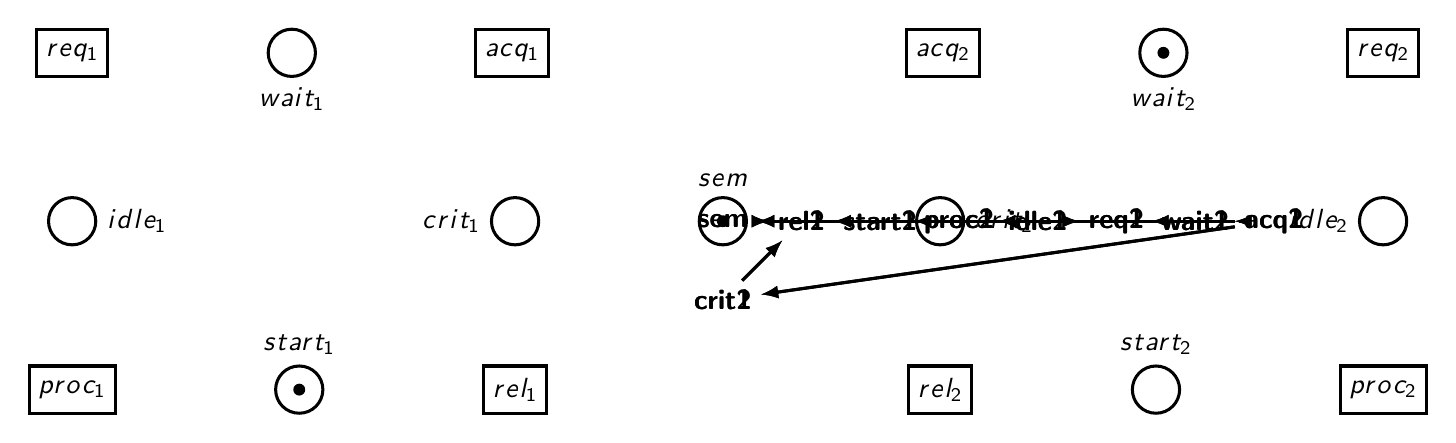
\begin{tikzpicture}
    % semaphor
    \node[place,tokens=1,label=above:$ sem $] (sem) {};

    % process 1 on the left
    \node[place,label=left:$ crit_1 $] (crit1) [left=of sem] {};
    \node[transition] (rel1) [below=of crit1] {$ rel_1 $};;
    \node[place,tokens=1,label=above:$ start_1 $] (start1) [left=of rel1] {};
    \node[transition] (proc1) [left=of start1] {$ proc_1 $};
    \node[place,label=right:$ idle_1 $] (idle1) [above= of proc1] {};
    \node[transition] (req1) [above=of idle1] {$ req_1 $};
    \node[place,label=below:$ wait_1 $] (wait1)  [right=of req1] {};
    \node[transition] (acq1) [right=of wait1]{$ acq_1 $};
    \graph{{sem,crit1} -> rel1 -> start1 -> proc1 -> idle1 -> req1 -> wait1 -> acq1 -> {sem,crit1}};

    % process 2 on the right
    \node[place,label=right:$ crit_2 $] (crit2) [right=of sem] {};
    \node[transition] (rel2) [below=of crit2] {$ rel_2 $};
    \node[place,label=above:$ start_2 $] (start2) [right=of rel2] {};
    \node[transition] (proc2) [right=of start2] {$ proc_2 $};
    \node[place,label=left:$ idle_2 $] (idle2) [above= of proc2] {};
    \node[transition] (req2) [above=of idle2] {$ req_2 $};
    \node[place,tokens=1,label=below:$ wait_2 $] (wait2)  [left=of req2] {};
    \node[transition] (acq2) [left=of wait2]{$ acq_2 $};
    \graph{{sem,crit2} -> rel2 -> start2 -> proc2 -> idle2 -> req2 -> wait2 -> acq2 -> {sem,crit2}};

    % \node[place, m3label={right}{$crit_2$}, module1copy, right=1.2cm of sem] (crit2) {};
    % \coordinate[offsetr] (center2);
    % \node[transition, below=of crit2, module1copy] (rel2) {$rel_2$};
    % \node[place, m3label={above}{$start_2$}, module1copy, right=of rel2] (start2) {};
    % \node[transition, right=of start2, module1copy] (proc2) {$proc_2$};
    % \node[place, m3label={left}{$idle_2$}, module1copy, right=of center2] (idle2) {};
    % \node[transition, above=of crit2, module1copy] (acq2) {$acq_2$};
    % \node[place, m3label={below}{$wait_2$}, module1copy, right=of acq2] (wait2) {}  {} [children are tokens] child {node[token, m3token] {}};
    % \node[transition, right=of wait2, module1copy] (req2) {$req_2$};
    % \graph[module1copy]{crit2 -> rel2 -> start2 -> proc2 -> idle2 -> req2 -> wait2 -> acq2 -> crit2 -> rel2};

\end{tikzpicture}
\end{document}